\documentclass[11pt]{article}
\usepackage[utf8]{inputenc}

%%%%%% LAYOUT %%%%%%%
\usepackage[margin=1in]{geometry} %Ask before changing or deleting this line.

%%%%%% USEFUL PACKAGES %%%%%%

\usepackage{amsmath,amssymb,amsfonts,amsthm}
\usepackage{enumitem}
\usepackage{multicol}

%%%%%% MAKING DIAGRAMS %%%%%%

\usepackage{asymptote} %Very powerful 
\usepackage{tikz} %Good for drawing graphs
\usepackage{graphicx} %Allows you to include external image files
\usepackage{ytableau} %Good for making Young tableaux
\usepackage{youngtab} %Good for making simple Young tableaux

%%%%%% USEFUL COMMANDS %%%%%%

%Feel free to add your own shorthands here.
\newcommand{\NN}{\mathbb{N}}
\newcommand{\ZZ}{\mathbb{Z}}
\newcommand{\RR}{\mathbb{R}}
\newcommand{\CC}{\mathbb{C}}
\newcommand{\QQ}{\mathbb{Q}}
\newcommand{\FF}{\mathbb{F}}
\newcommand{\PP}{\mathbb{P}}


\newtheorem{theorem}{Theorem}
\newtheorem{prop}[theorem]{Proposition}
\newtheorem{corollary}[theorem]{Corollary}
\newtheorem{lemma}[theorem]{Lemma}
\newtheorem{conjecture}[theorem]{Conjecture}

\theoremstyle{definition}

\newtheorem{definition}[theorem]{Definition}
\newtheorem{remark}[theorem]{Remark}
\newtheorem{example}[theorem]{Example}

\numberwithin{theorem}{section}



%%%%% TITLE, AUTHOR %%%%%

\title{\vspace{-2.7cm}Moduli Spaces of Stable Curves with Marked Points: Examples and Connections to Trees.\vspace{-0.7cm}}
\author{Ignacio Rojas}
\date{Spring, 2023}


\begin{document}

\maketitle{}

\begin{abstract}
    \vspace*{-1.5em}
    This work explores the concept of moduli spaces of stable curves with marked points, which are sets of parameters describing families of objects. These spaces can be used to solve problems in enumerative geometry, such as determining the number of curves passing through a given number of points. The common principle underlying these solutions is the association of the objects with a moduli space, which provides a different perspective on the problem. We illustrate this connection with examples.
    \end{abstract}
    
    \begin{flushleft}
    \small
    \emph{Keywords}:
    moduli space, curves enumerative geometry, parametrization.
    
    \emph{MSC classes}:  Primary \texttt{14D22}; Secondary \texttt{05C05, 14H10}.
    \end{flushleft}
    
\section{Introduction}

Let us begin with a simple question:
\begin{significant}
Which are the quadratic curves which pass through $4$ points in $\bR^2$ and no three of them are collinear?
\end{significant}
This question might be a bit tough to tackle right now, but let us simplify. How about if the points are $(1,1),(1,-1),(-1,-1)$ and $(-1,1)$? At once the following idea should pop-in in our heads: \emph{a circle}! The circle which passes through these points is described by the equation $x^2+y^2=2$ as seen in Figure \ref{fig1}.
\begin{figure}[h!]
    \centering
    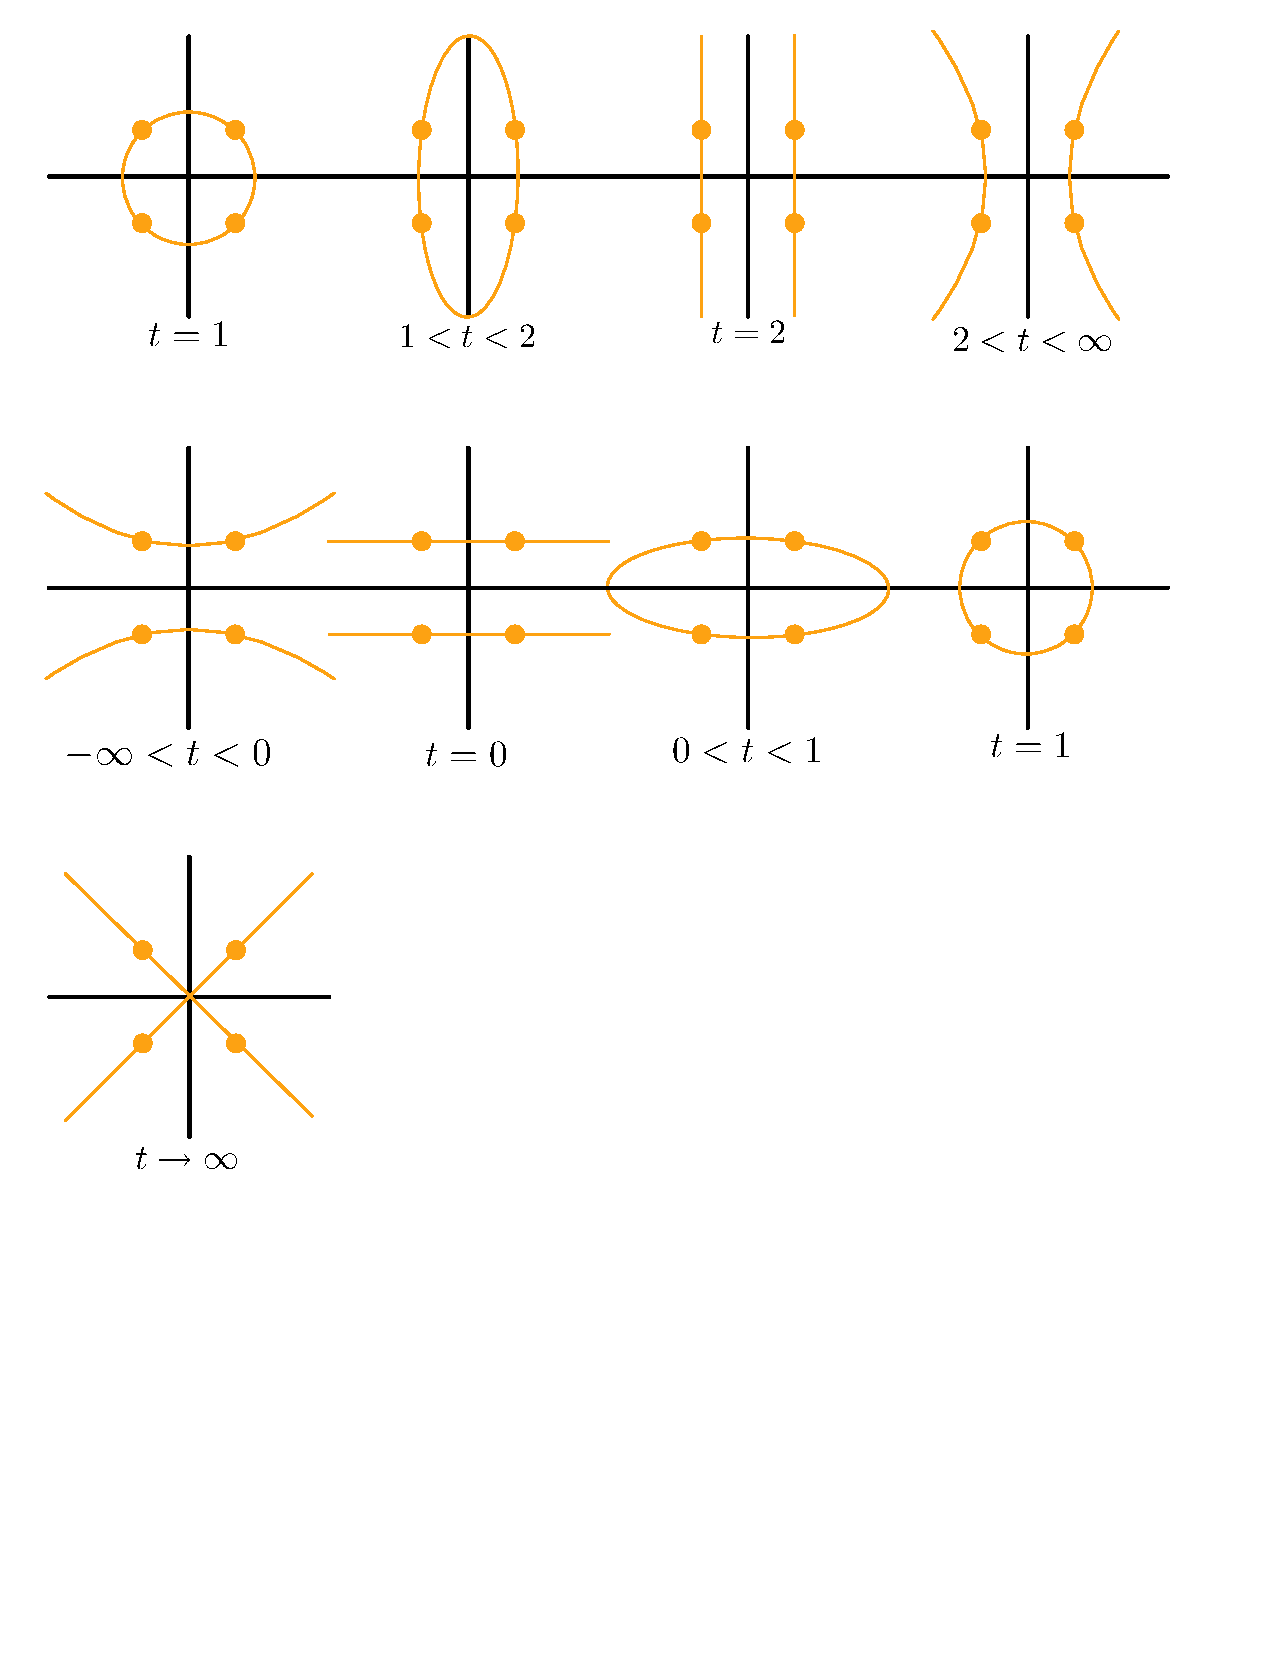
\includegraphics[width=0.3\textwidth, trim= 0.8cm 22.9cm 16cm 0.6cm,clip]{fig1.pdf}
    \label{fig1}
    \caption{One of the quadratic curves passing through our points: $x^2+y^2=2$.}
\end{figure}
Ideally we would like to stretch and shrink the circle in order to make it an ellipse. We know ellipses have equations of the form $x^2/a^2+y^2/b^2=1$, but to begin from our circle equation we will instead add coefficients to the equation 
$$Ax^2+By^2=2.$$
These coefficients are determined by the points on the curve, we may derive the relation by plugging in a point into the equation:
$$A(1)^2+B(1)^2=2\To B=2-A\To tx^2+(2-t)y^2=2$$
where we take $t=A$ to get the last equation.
We annotate the curves we obtain given different values of $t$:
\vspace{-0.5em}
\begin{itemize}
    \begin{multicols}{2}
        \itemsep=-0.4em
    \item $(t=1)$: A circle.
    \item $(1<t<2)$: An ellipse.
    \item $(t=2)$: The pair of lines $x^2=1$.
    \item $(t>2)$: A hyperbola.
    \end{multicols}
\end{itemize}
However we are left with one curve which passes through the points in question. To find it we will assume $t$ is non-zero. From our parametric equation we obtain 
$$tx^2+(2-t)y^2=2\To x^2+o(t^2)+y^2=\frac{2}{t^2}\xrightarrow[t\to\infty]{}x^2=y^2$$
which is the pair of lines $y=\pm x$. Observe that this behavior is independent of the sign of the infinity we are going to. 
\begin{figure}[h!]
    \centering
    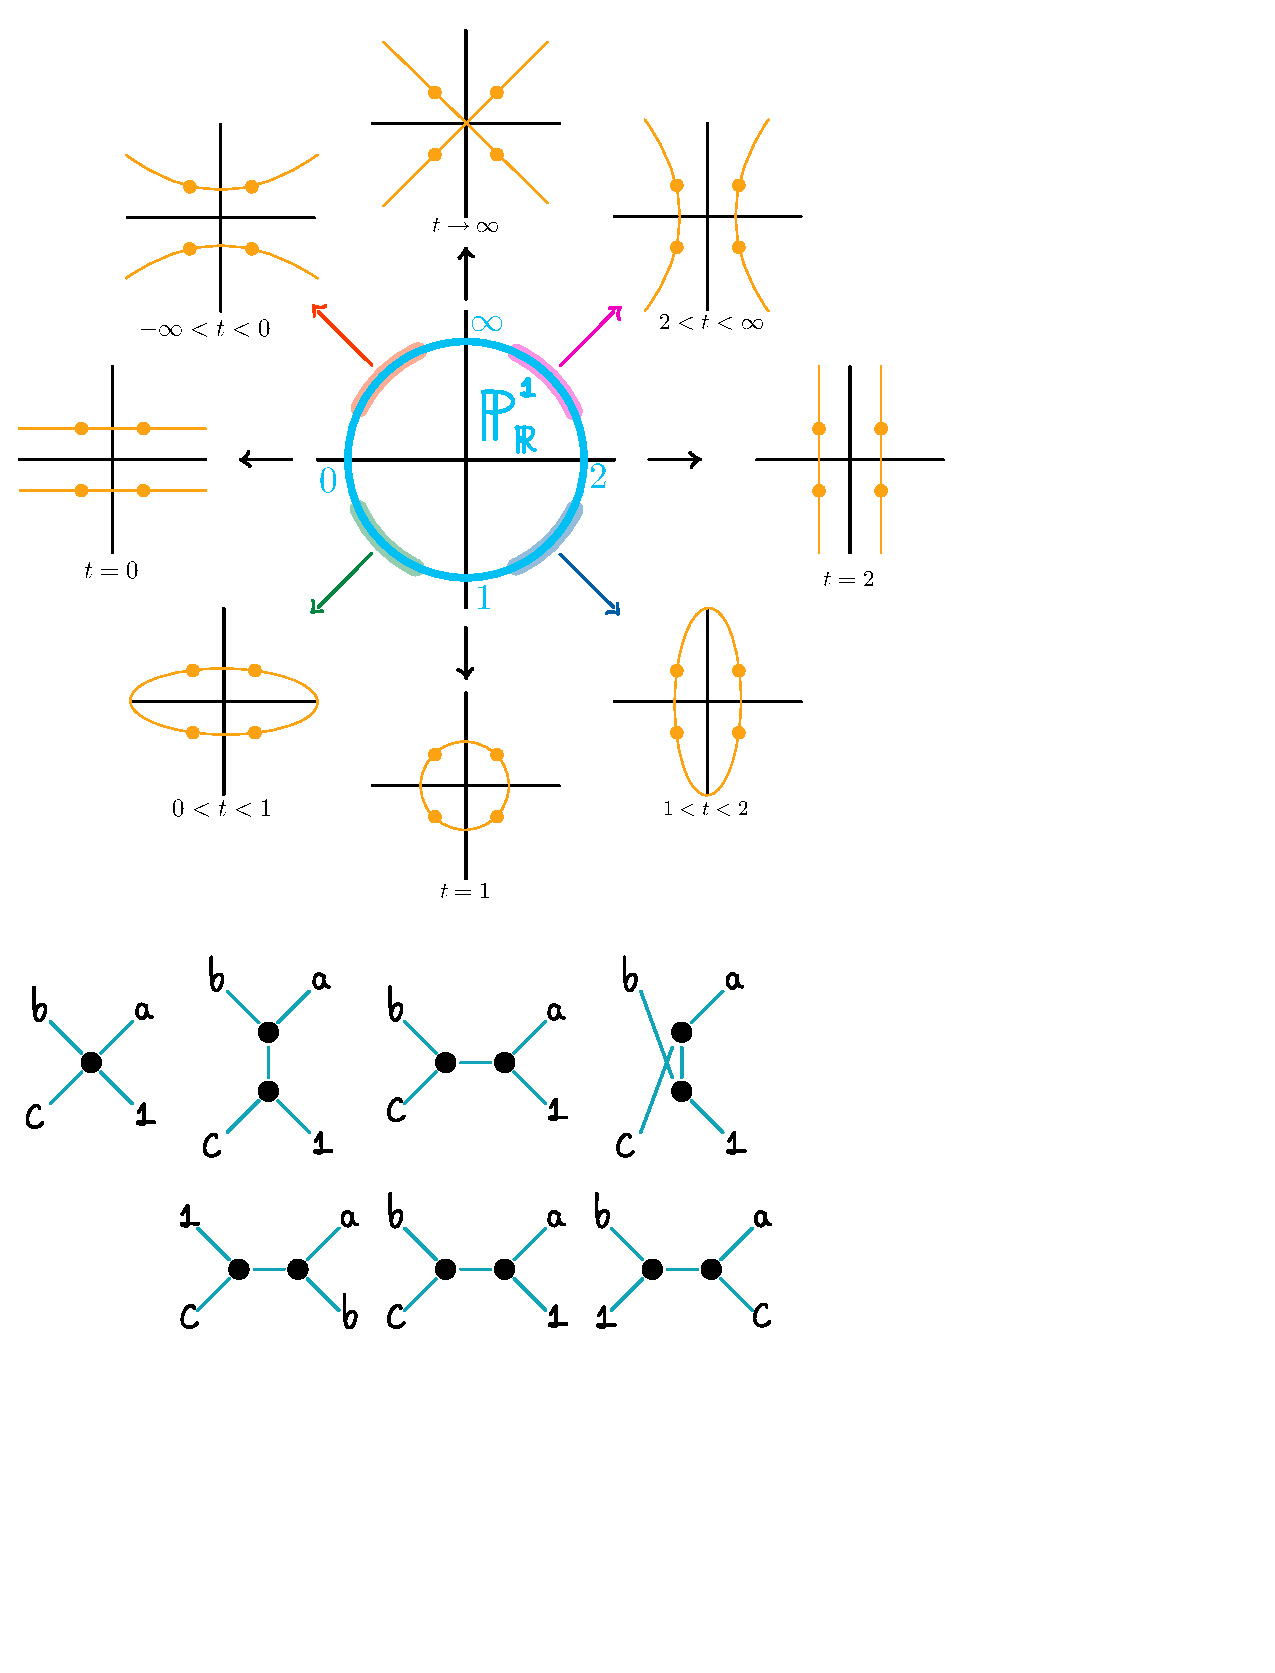
\includegraphics[width=0.8\textwidth, trim= 0.25cm 13.1cm 5.25cm 0.5cm,clip]{fig2.pdf}
    \label{fig2}
    \caption{The projective real line as the moduli space $\ov\cM_{0,4}$.}
\end{figure}
In essence what we have seen is that all the quadratic curves passing through our set of points can be parametrized by $\bR\cup\set{\infty}$. Formally:
\begin{Prop}
The moduli space $\ov{\cM}_{0,4}$ can be identified with $\bP^1_\bR$.
\end{Prop}
Intuitively the \term{moduli space} is a set of parameters. When the points vary \emph{continuously}, the objects they parametrize deform \emph{continuously} as well. What we have done here is not a proof of the previous proposition but it may serve as evidence that it is true.\par 
To study this space and other spaces which may arise in this fashion, we may ask a question like \emph{how many such curves can we find?} In order to do this, we will address this problem by connecting it with graphs. 

\section{Connection with trees}

\section{Open Problems}

There are a number of interesting open problems remaining to be solved in this area.  For instance, the following is the statement of the Confusing Conjecture \cite{FancyGuy}.

\begin{conjecture}
  The Confusing Conjecture.
\end{conjecture}


\section{Further Observations}

In this section we list several further observations that we made on this topic.  

In Sage, we checked that the Confusing Conjecture does indeed hold for all $n\le 7$.  This was in fact checked up to $n\le 9$ by [citation], but we also verify the following subcase for $n=10$:

\begin{example}
    Subcase for $n=10$.
\end{example}

%%%%%You can of course have as many sections as you need to organize your ideas clearly.

%%%%%% BIBLIOGRAPHY %%%%%%

%You may use bibtex if you prefer, but here is a simple way of creating your bibliography:

\begin{thebibliography}{99}
\bibitem{Stanley} R.~Stanley, \textit{Enumerative Combinatorics, Vol. 2}, Cambridge University Press, Cambridge (1999).

\bibitem{Fulton} W.~Fulton, \textit{Young tableaux: with applications to representation theory and geometry}, Cambridge University Press (2012). 

\bibitem{FancyPerson} Some Famous Mathematician, On a Scary-Sounding Title with Several Adjectives, \textit{Journal of High Impact}, Vol. 3 (1992).

\end{thebibliography}


\end{document}